\section{Escenarios de Uso Frecuente}
\label{sec:escenarios_uso}

En esta sección se analizan en detalle tres escenarios representativos en los cuales HTTPS y los protocolos criptográficos asociados desempeñan un rol crítico. Para cada escenario se proporciona: (i) una descripción funcional; (ii) un diagrama ilustrativo (exportado desde Mermaid); (iii) un análisis de amenazas y contramedidas; (iv) recomendaciones de configuración y buenas prácticas; y (v) un checklist operativo para despliegues reales. Las referencias citadas apoyan las recomendaciones técnicas empleadas (\cite{rfc8446, rfc7525, sasse2023, nikiforakis2012}).

\subsection{Escenario 1: Comercio Electrónico y Servicios Bancarios en Línea}
\label{subsec:escenario_comercio_banca}

\begin{figure}[H]
    \centering
    % Sustituye por tu diagrama exportado desde mermaid (por ejemplo: figuras/escenario_comercio.pdf)
    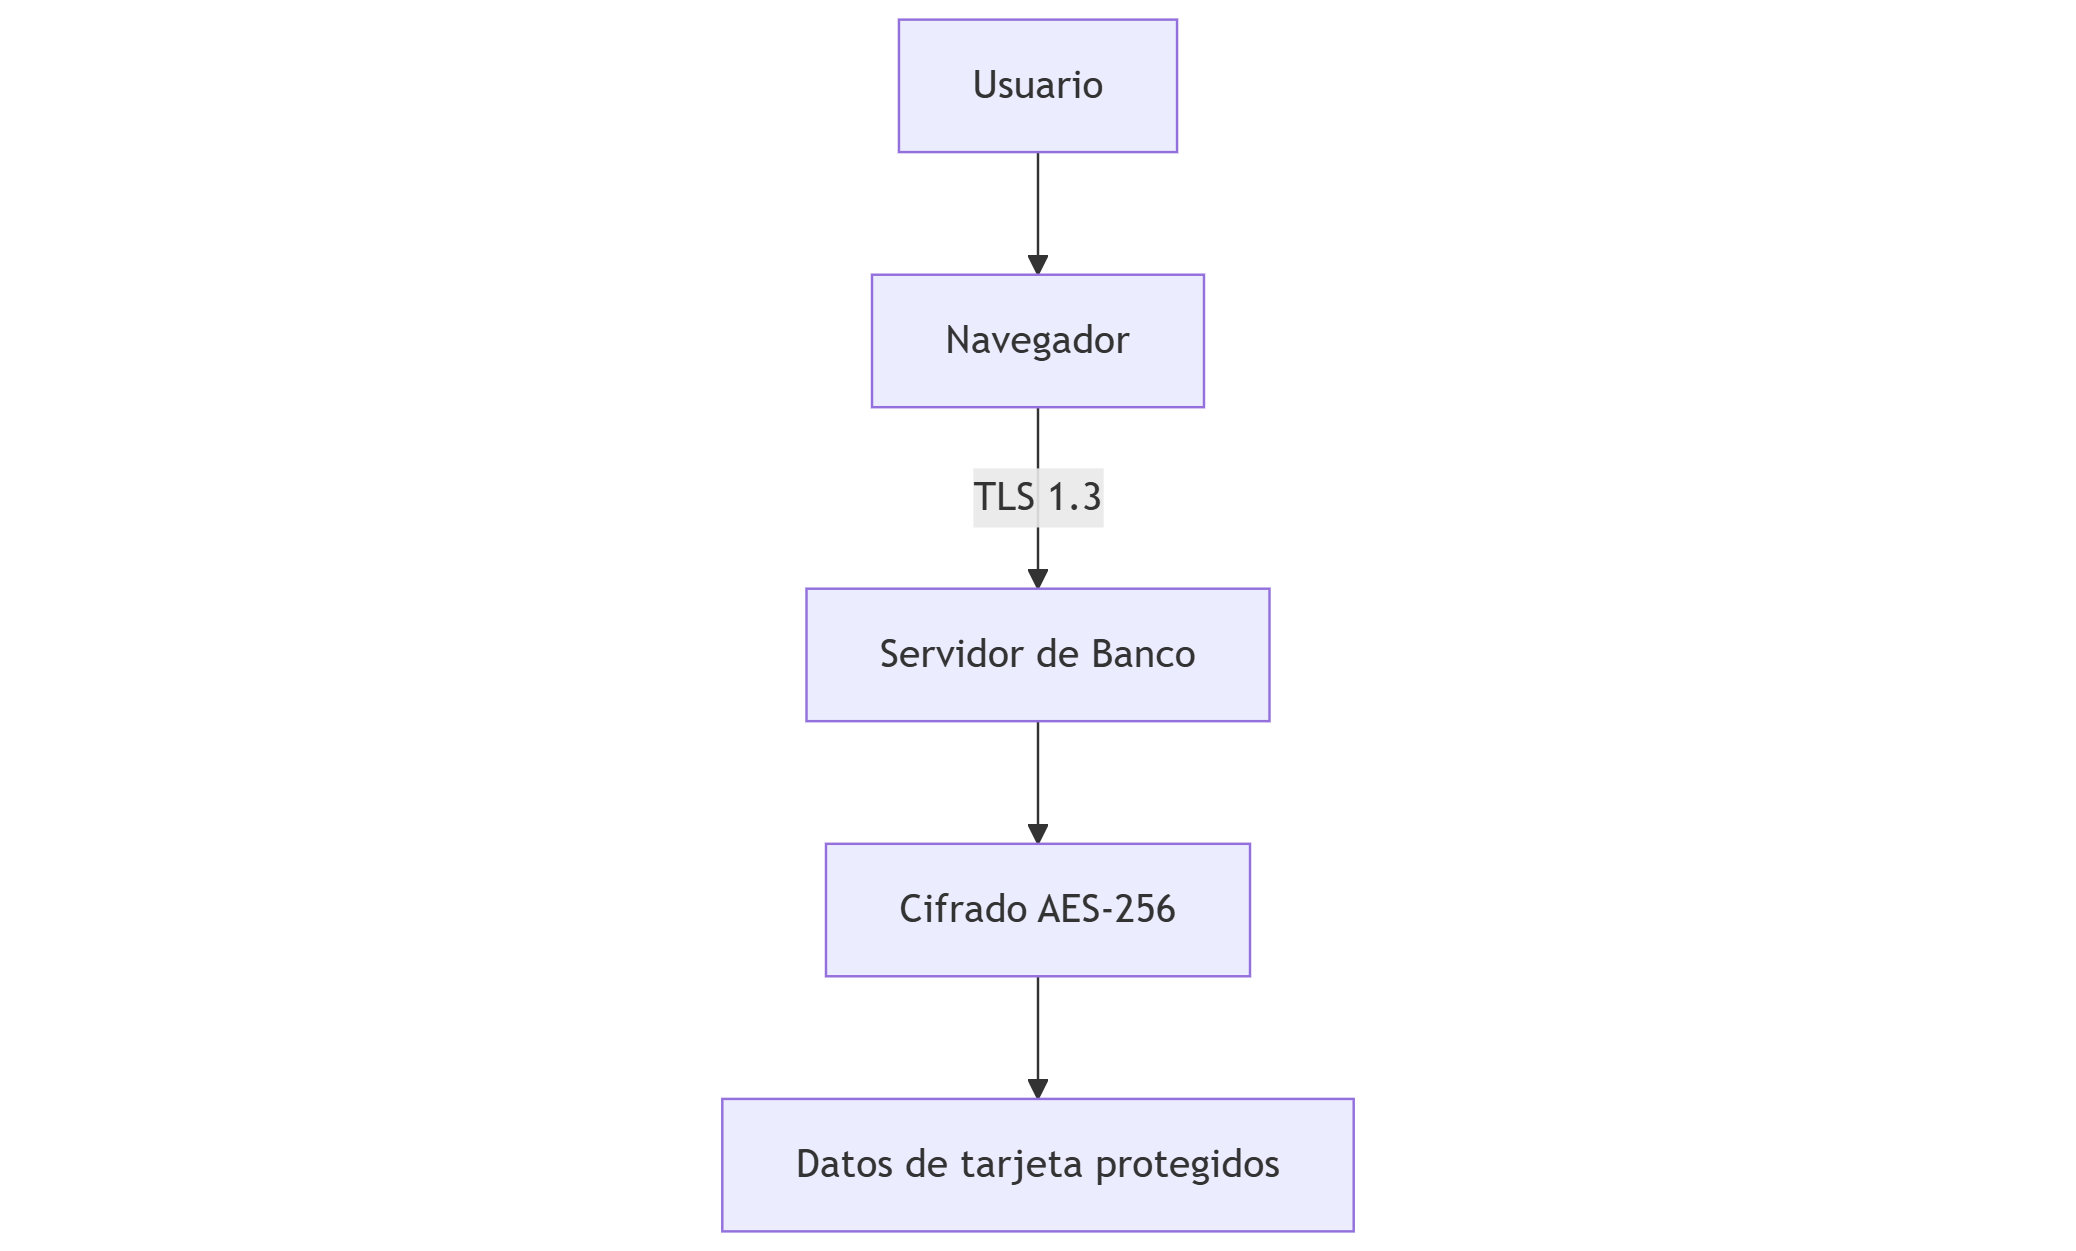
\includegraphics[width=0.9\textwidth]{assets/images/mermaid-diagram-2025-11-29-194541.png}
    \caption{Arquitectura típica de comercio electrónico: cliente, gateway de pago, servidor de aplicación y capa de pago externa.}
    \label{fig:escenario_comercio}
\end{figure}

\paragraph{Descripción funcional.}  
En plataformas de comercio electrónico y banca en línea, HTTPS protege la comunicación entre el cliente (navegador o aplicación móvil) y los servicios back-end que procesan credenciales y transacciones financieras. El flujo habitual incluye navegador $\rightarrow$ servidor web (TLS) $\rightarrow$ API interna $\rightarrow$ pasarela de pago (tercera parte), donde cada salto debe utilizar canales cifrados y autenticados. La protección incluye cifrado de sesión (AES-GCM/ChaCha20-Poly1305), autenticación de servidor mediante certificados X.509 y, cuando procede, autenticación fuerte del usuario (MFA) sobre el canal seguro \cite{rfc8446}.

\paragraph{Principales amenazas y mitigaciones.}
\begin{itemize}
    \item \textbf{Intercepción de credenciales y datos de pago (MITM).} Mitigación: TLS 1.3 con suites AEAD, HSTS y uso de certificados emitidos por CAs de confianza. Implementar Certificate Transparency y monitorización de certificados anómalos.
    \item \textbf{Reutilización de sesiones o ataques de replay.} Mitigación: claves efímeras (ECDHE) para PFS, tokens de un solo uso (OTP) y expiración corta de sesiones.
    \item \textbf{Inyección/alteración en recursos de terceros (third-party content).} Mitigación: evitar incluir recursos inseguros; usar subresource integrity (SRI) y servir dependencias desde HTTPS confiable \cite{nikiforakis2012}.
    \item \textbf{Fugas por configuración TLS débil (cipher suites obsoletas).} Mitigación: configuración restrictiva que priorice ECDHE+AEAD y deshabilite RC4, 3DES, y suites basadas en RSA key-exchange \cite{rfc7525}.
\end{itemize}

\paragraph{Recomendaciones de configuración (producción).}
\begin{itemize}
    \item Forzar TLS 1.3 y mantener compatibilidad controlada con TLS 1.2 sólo si es estrictamente necesario.
    \item Habilitar HSTS con periodo largo y preloading donde aplique.
    \item Implementar OCSP Stapling para mejorar la latencia y privacidad en la validación de revocación.
    \item Usar certificados emitidos por CAs reconocidas y, para servicios críticos, considerar certificados con short-lived validity o automatización ACME (Let's Encrypt) junto con gestión de rotación.
    \item Aislar la clave privada: almacén seguro o HSM; permisos de fichero mínimos en servidores.
    \item Implementar detección y respuesta a incidentes (logs de handshake, alertas por cambios de certificado).
\end{itemize}

\paragraph{Checklist operativo (rápido).}
\begin{enumerate}
    \item TLS 1.3 habilitado, AEAD suites preferidas.
    \item HSTS con \texttt{includeSubDomains} y \texttt{preload} cuando corresponda.
    \item OCSP Stapling activo.
    \item Rotación y backup de claves privadas; HSM para entornos regulados.
    \item Pruebas periódicas con \texttt{testssl.sh} o SSL Labs.
    \item Revisión de terceros y bloqueo de recursos inseguros (SRI).
\end{enumerate}

\paragraph{Cumplimiento y consideraciones regulatorias.}  
Para plataformas que procesan datos de pago se recomienda el alineamiento con PCI-DSS (requisitos relativos a cifrado en tránsito), así como el registro de auditorías que demuestren la correcta configuración de TLS y la gestión de claves. Estas prácticas reducen riesgo regulatorio y mejoran la confianza del usuario.

\subsection{Escenario 2: Correo Electrónico Seguro (SMTP/IMAP/POP3 sobre TLS)}
\label{subsec:escenario_correo}

\begin{figure}[H]
    \centering
    % Sustituye por tu diagrama exportado desde mermaid (por ejemplo: figuras/escenario_correo.pdf)
    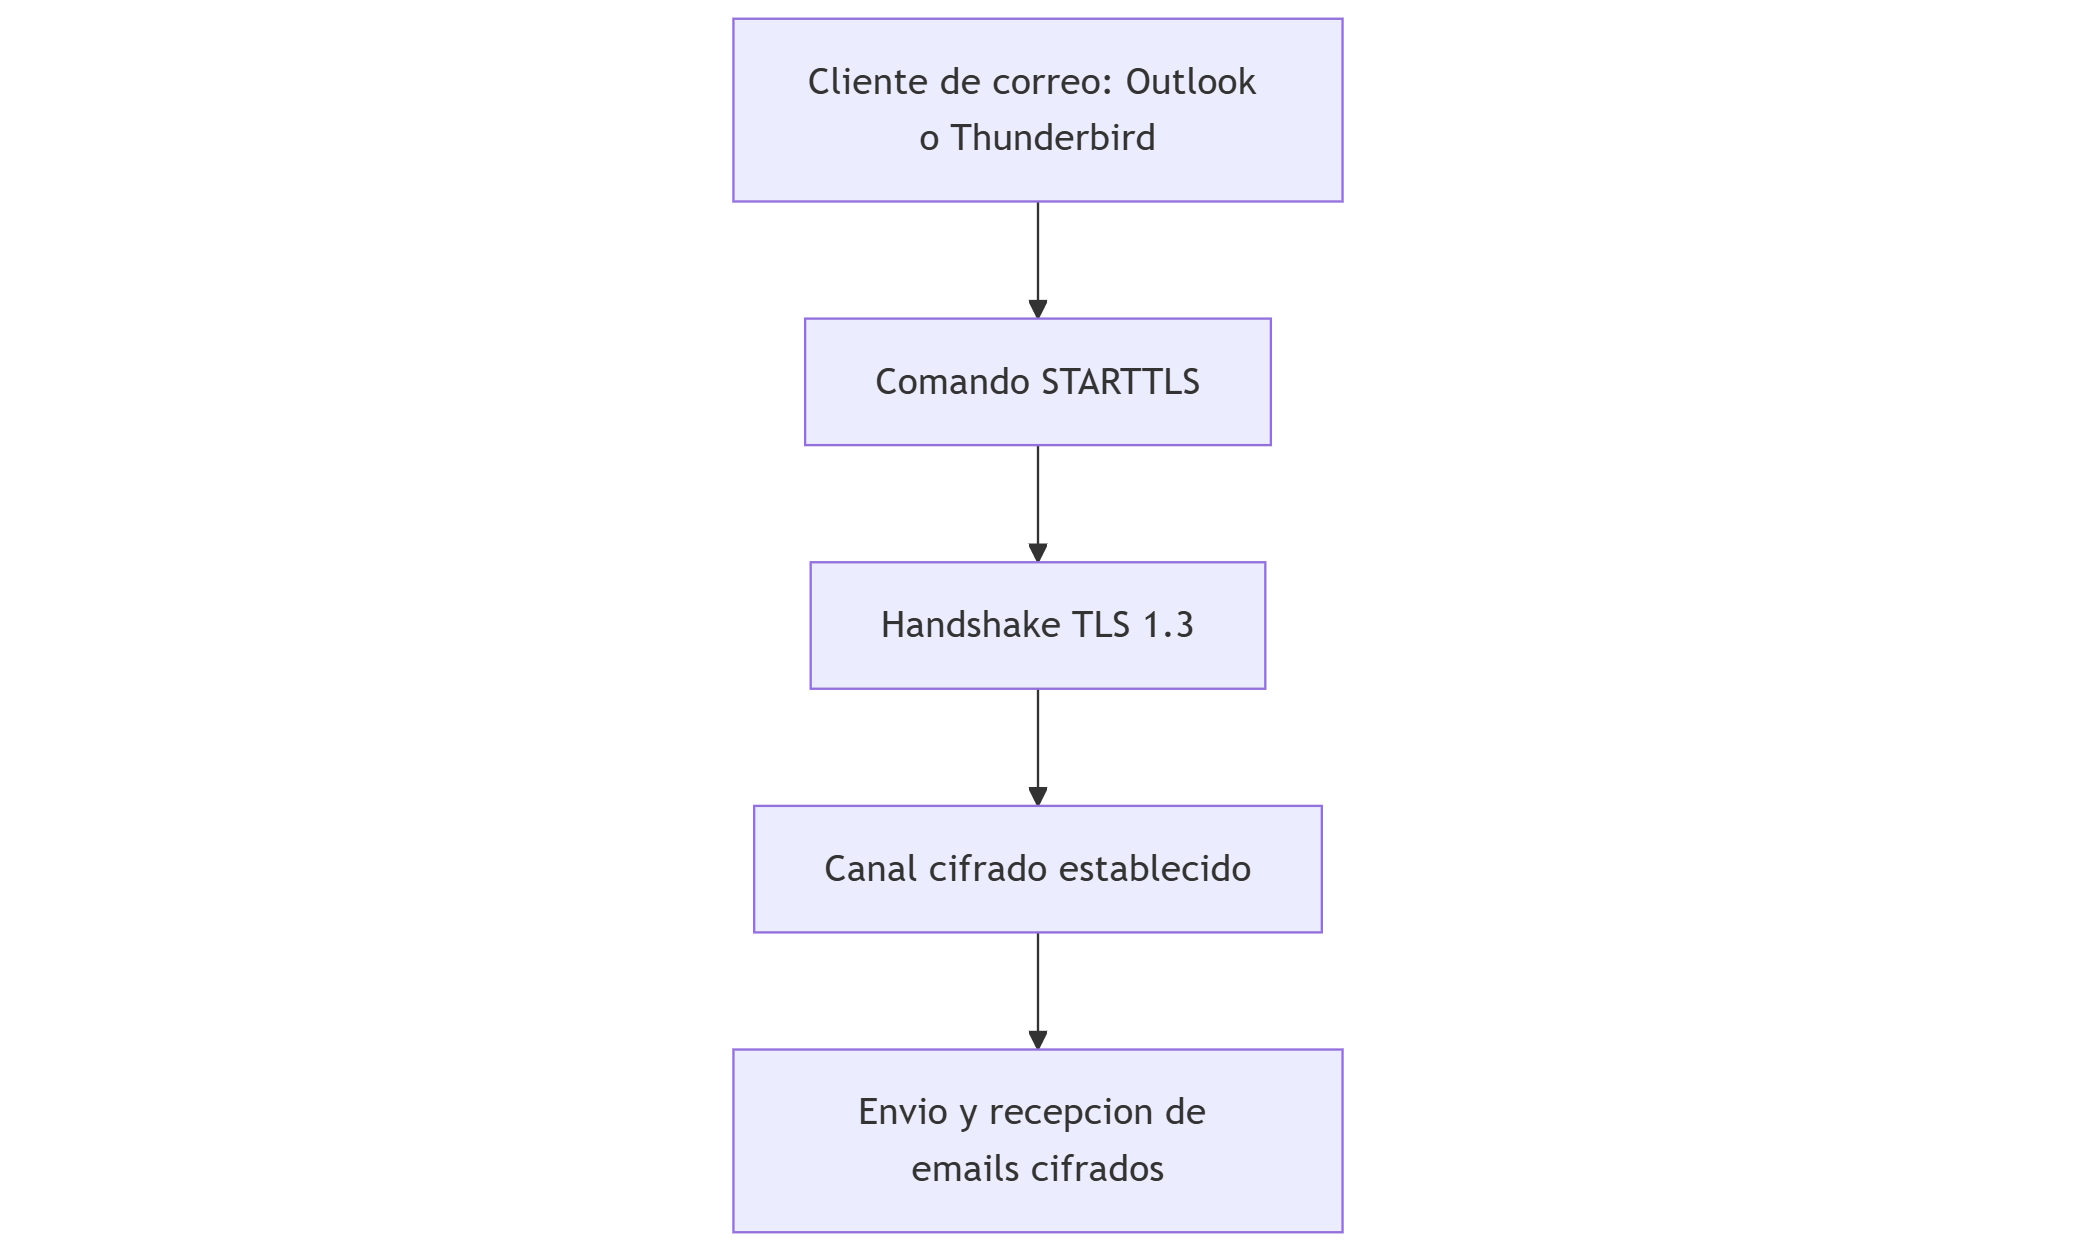
\includegraphics[width=0.85\textwidth]{assets/images/mermaid-diagram-2025-11-29-194948.png}
    \caption{Topología de correo: cliente de correo, servidor MTA/IMAP y utilización de STARTTLS/SMTPS para asegurar canales.}
    \label{fig:escenario_correo}
\end{figure}

\paragraph{Descripción funcional.}  
El ecosistema de correo electrónico se sustenta en protocolos como SMTP, IMAP y POP3; para asegurar estos canales se utiliza TLS (SMTPS/IMAPS/POP3S) o el mecanismo STARTTLS que eleva una conexión cleartext a cifrada. La adopción de TLS protege la confidencialidad de contenidos y credenciales en tránsito entre clientes y servidores, y entre servidores remitentes/receptores cuando se negocia TLS en MTA-to-MTA \cite{rfc8446}.

\paragraph{Principales amenazas y mitigaciones.}
\begin{itemize}
    \item \textbf{Downgrade y ataques de stripping en STARTTLS.} Mitigación: políticas estrictas de MTA (MTA-STS), DANE (DNS-based Authentication of Named Entities) cuando sea viable, y configuración que favorezca SMTPS sobre STARTTLS en enlaces críticos.
    \item \textbf{Intercepción de credenciales en tránsito.} Mitigación: uso forzado de TLS para clientes y servidores, implementación de SASL sobre TLS y rechazo de autenticaciones en canales no cifrados.
    \item \textbf{Phishing y spoofing por certificados fraudulentos.} Mitigación: validación estricta de cadenas de confianza, monitorización de certificados y estrategias de reputación.
\end{itemize}

\paragraph{Recomendaciones de configuración.}
\begin{itemize}
    \item Preferir conexiones TLS directas (SMTPS/IMAPS) y usar STARTTLS sólo con políticas de MTA-STS o DANE.
    \item Implementar autenticación fuerte (SASL mechanisms como SCRAM) sobre TLS.
    \item Habilitar TLS en enlaces MTA-to-MTA y lanzar alertas ante caídas de cifrado.
    \item Usar certificados válidos y rotación periódica; OCSP Stapling para MTA cuando sea soportado.
\end{itemize}

\paragraph{Checklist operativo.}
\begin{enumerate}
    \item Configurar MTA para requerir TLS en conexiones salientes/entrantes según la política.
    \item Habilitar MTA-STS y evaluar DANE si el dominio lo permite.
    \item Forzar autenticación SASL sobre TLS.
    \item Monitorear retransmisiones fallidas y negociaciones sin cifrado.
\end{enumerate}

\subsection{Escenario 3: APIs RESTful y Arquitecturas de Microservicios}
\label{subsec:escenario_apis_microservicios}

\begin{figure}[H]
    \centering
    % Sustituye por tu diagrama exportado desde mermaid (por ejemplo: figuras/escenario_apis.pdf)
    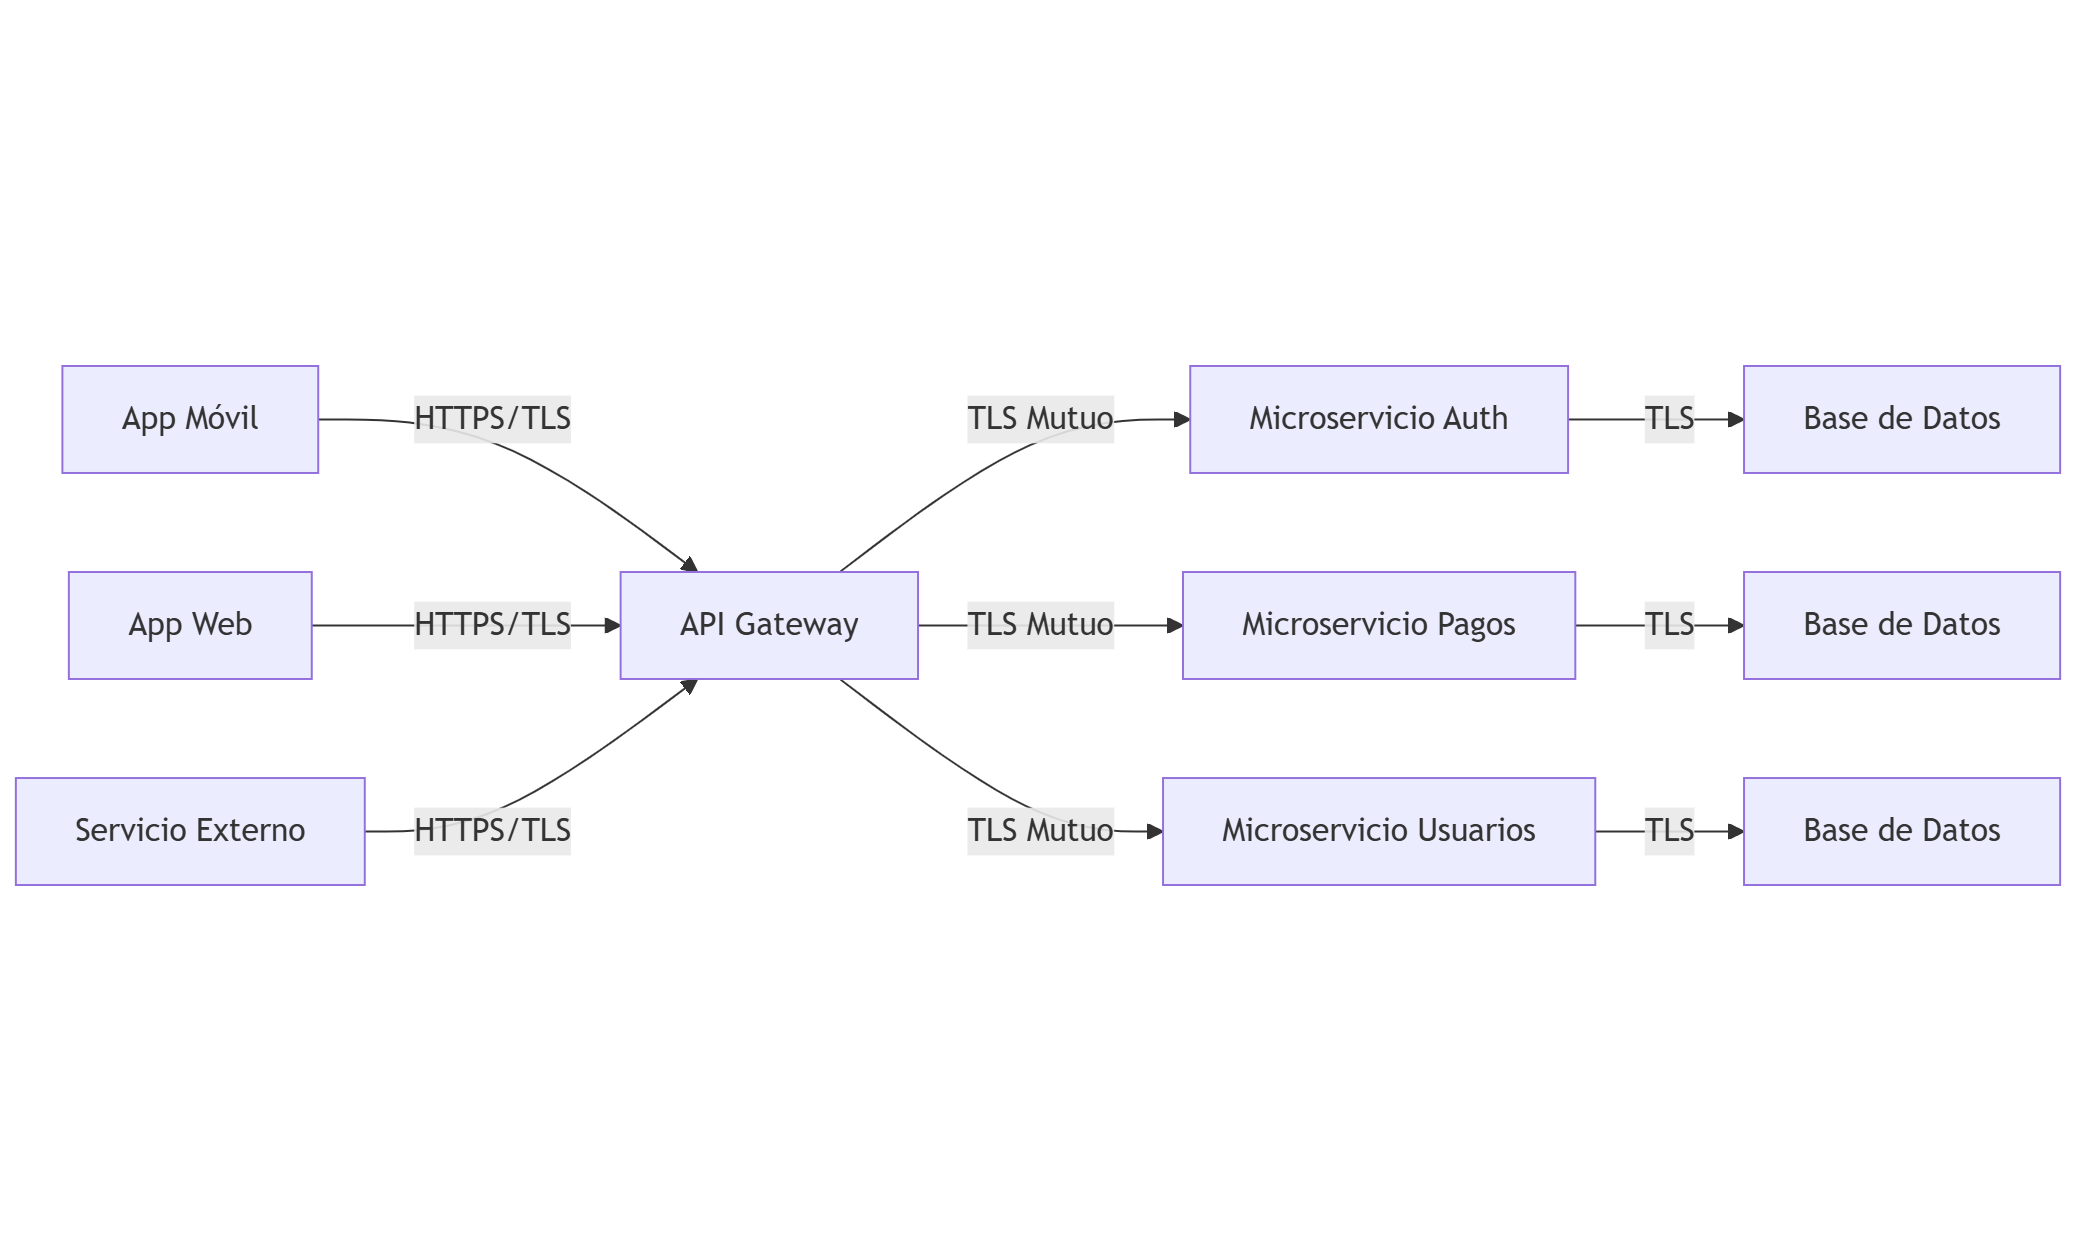
\includegraphics[width=0.9\textwidth]{assets/images/mermaid-diagram-2025-11-29-195055.png}
    \caption{Arquitectura típica de APIs y microservicios con API Gateway, mTLS entre servicios y almacenamiento backend protegido.}
    \label{fig:escenario_apis}
\end{figure}

\paragraph{Descripción funcional.}  
En arquitecturas modernas, las APIs RESTful son el vehiculo principal de comunicación entre clientes y servicios, y entre microservicios internos. HTTPS protege tanto el acceso expuesto al exterior (cliente $\rightarrow$ API Gateway) como las comunicaciones internas (microservicio $\leftrightarrow$ microservicio). En entornos sensibles se emplea \emph{mutual TLS} (mTLS) para autenticar y autorizar de forma mutua los endpoints, reduciendo la necesidad de confiar en credenciales estáticas y mitigando ataques laterales \cite{sasse2023}.

\paragraph{Principales amenazas y mitigaciones.}
\begin{itemize}
    \item \textbf{Compromiso lateral entre servicios (east–west attacks).} Mitigación: mTLS, segmentación de red, políticas de autorización y verificación de identidad por servicio.
    \item \textbf{Fuga de credenciales y tokens en cabeceras.} Mitigación: transmitir tokens sólo sobre HTTPS, uso de short-lived JWTs y verificación de revocación/blacklist.
    \item \textbf{Inyección de dependencias remotas y contenido no confiable.} Mitigación: validar y sanear entradas, aplicar políticas de CORS estrictas y evitar incluir recursos de terceros sin control \cite{nikiforakis2012}.
\end{itemize}

\paragraph{Recomendaciones de configuración y diseño.}
\begin{itemize}
    \item Implementar mTLS para comunicaciones internas entre servicios críticos; automatizar la emisión/rotación de certificados mediante una PKI interna o soluciones como Istio/Consul.
    \item Forzar HTTPS en el borde (API Gateway) y aplicar políticas de rate limiting, WAF y autenticación fuerte (OAuth2/OpenID Connect).
    \item Emplear certificate pinning en aplicaciones móviles cuando se justifique, con procedimientos de actualización controlados.
    \item Monitorizar telemetría de handshakes TLS y latencias para detectar anomalías o intentos de degradación.
\end{itemize}

\paragraph{Checklist operativo (microservicios).}
\begin{enumerate}
    \item mTLS habilitado y gestionado por una PKI interna (rotación automática).
    \item API Gateway con TLS 1.3, WAF y políticas de autenticación (OAuth2).
    \item Tokens de acceso short-lived y validación server-side.
    \item Observabilidad: métricas TLS, logs de handshake, y alertas por fallos de validación.
\end{enumerate}

\subsection{Consideraciones transversales}
\label{subsec:consideraciones_transversales}

Al margen de las particularidades de cada escenario, se deben considerar prácticas transversales que aumentan la resiliencia global:

\begin{itemize}
    \item \textbf{Automatización de certificados:} uso de ACME/Let’s Encrypt para certificados públicos y sistemas internos de entrega para PKI privada.
    \item \textbf{Pruebas continuas y auditoría:} integración de herramientas como \texttt{testssl.sh}, SSL Labs y scanners de seguridad en pipelines de CI/CD.
    \item \textbf{Políticas de actualización:} vigilar CVE y actualizaciones de bibliotecas criptográficas (OpenSSL, BoringSSL, NSS).
    \item \textbf{Gestión de revocación:} evaluar OCSP Stapling y short-lived certificates para minimizar problemas de revocación observados en la práctica \cite{liu2015, helme2024}.
\end{itemize}

\noindent\textbf{Referencias.} Las prácticas y recomendaciones aquí descritas se basan en las especificaciones y estudios citados en la bibliografía, que incluyen análisis formales del protocolo TLS y evaluaciones empíricas de la infraestructura PKI a escala global \cite{rfc8446, rfc7525, liu2015, helme2024, sasse2023, nikiforakis2012}.

